
\documentclass[main.tex]{subfiles}
\begin{document}
% Бла, бла, бла, аз съм толкова емоционална. 
% Не знам

% 
\includegraphics[width=0.5\textwidth ]{pikachu}
Много хора си мислят, че в началото бе Словото. Всъщност, 
\begin{displayquote}
    В началато бе създадена Вселената. Този факт разгневи силно много хора и сега се шири мнението, че това е била погрешна стъпка.\footnote{Ресторант „На края на Вселената“ от Дъглас Адамс}
\end{displayquote}
    
След това дойде словото.

Словото, и по-точно говоримата реч, все още е най-ефективният метод за предаване на информация между хора. Това е така, защото речта е изключително удобна за тази цел. От една страна защото е естествена, в смисъл на ``хората са анатомично предразположени да произвеждат реч''. От друга, може да се комуникира, без да има нужда от директен зрителен контакт, на малки или сравнително големи разстояния. Ако ситуацията позволява, може да се кодира и допълнително информация. Обикновено когато се говори за реч, се различават два компонента. Единият, \textbf{очевидният}, е словесният, който предава експлицитно съобщение. Вторият е компонентът на прозодията. Прозодията се отнася до елементи на речта като интонация, тон, ритъм и ударение. Чрез нея се кодира допълнителна информация, която не може да се предаде чрез граматика или писмен вид. Прозодията може да определя дали изречението е въпросително или е повелително, дали е иронично или саркастично. Най-вече, по този начин се кодира имплицитна информация за говорещия и неговото емоционално състояние. Добавянето на този канал към комуникацията я прави значително по-богата и много по-ефективна. В много ситуации, без информация за прозодията на някакво изказване, дори не може да се предаде съобщението му (\autoref{fig:intro:1}). Поради тази причина, всяко приложение, използващо човешка реч, е желателно да се възползва и от информацията, кодирана в прозодията. Хората са много чувствителни към нея. Показано е в \cite{urgency}, че има голяма разлика във възприетата важност на съобщението в зависимост от интонацията, както и че например пилотите предпочитат човешки пред компютърен глас при предаване на важни съобщения\footnote{Интересен факт: жаргонният израз за женски глас, използван за предупредително съобщения в самолети, е ``Bitching Betty''} \cite{cockpit}. Тъй като голяма част от прозодията кодира информация за емоционалното състояние на говорещият, разпознаването на емоцията в сигнали е интересен (за мен) въпрос.

Съществуват много изследвания в областта на разпознаването на емоции от мозъчни вълни, както и съществуват много мулти-модални системи, които съчетават вторични изрази като реч, визуални данни, термални данни и други. Наличието на подръчен електроенцефалограф, лесното създаване на аудио данни и естественото любопитсвто, вдъхновиха опита за съчетаване на един първичен канал - сигнал от електроенцефалографа - и един вторичен - сигнал от реч. Въпросът, който се разглежда, е до какво ще доведе съчетаването на тези два сигнала, при разпознаването на емоции в тях. Текстът на дипломната работа е разделен на значещите части на заглавието ѝ както следва:
\begin{itemize}
    \item В \autoref{chap:emotion} е описано какво все пак имаме предвид под емоция и какво точно целим да разпознаваме
    \item В \autoref{chap:speech} е описан физичния процес на производство на реч и характеристичните вектори, които ще извличаме от този сигнал, както и класификационни резултати само от този сигнал
    \item В \autoref{chap:eeg} са описани (много по-малко подробно) спецификите на извличане на характеристични вектори от ЕЕГ сигнал, както и класификационни резултати само от него
    \item В \autoref{chap:double} се описват методи за съчетаване на двата сигнала и резултатът от това
    \item Накрая заключението е изложено в \nameref{conclusion} 
\end{itemize}
\begin{center}
    \begin{figure}[ht]%
        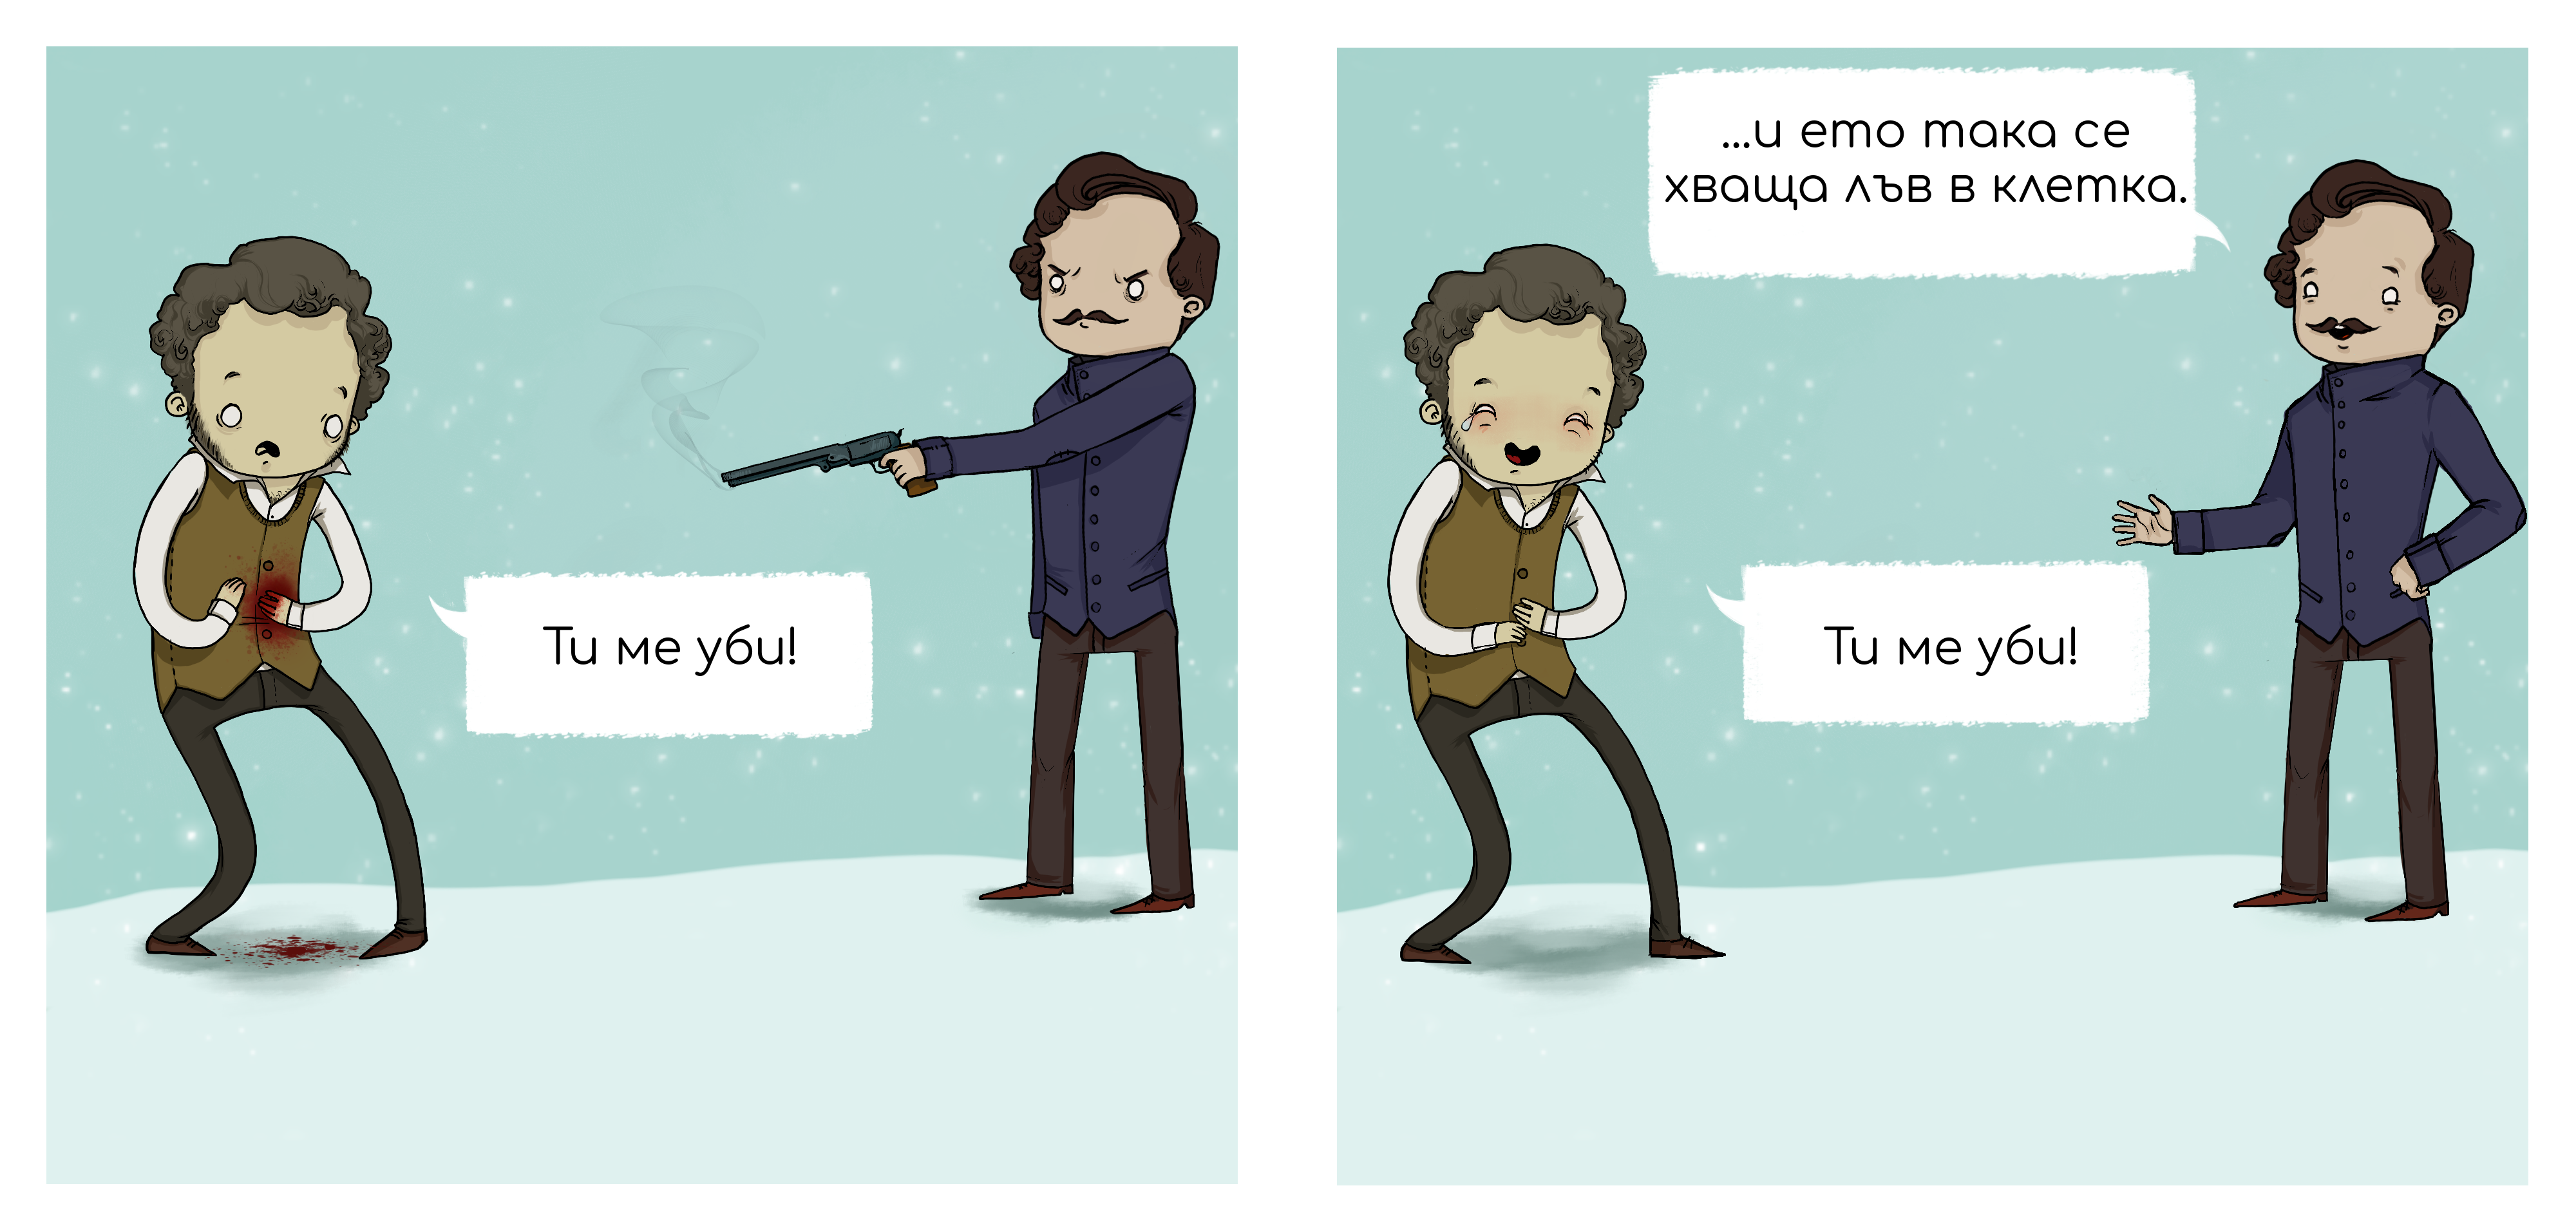
\includegraphics[width=\textwidth]{meaning.png}%
        \caption{Пример за многозначност на изказване, която не може да бъде разрешена, без да се предаде допълнителелна информация.}%
        \label{fig:intro:1}
    \end{figure}
\end{center}

\let\thefootnote\relax\footnotetext{Попълването на вица е оставено за упражнение на читателя}

\end{document}